% Cartoon pint of stout for the slide "Student's t-test: a brewery story".
% Compile from class3/:  pdflatex pint_glass.tex
%   then: pdftocairo -png -transp -singlefile -scale-to-x 800 -scale-to-y -1 pint_glass.pdf img/pint_glass
\documentclass[tikz,border=4pt]{standalone}
\usepackage[T1]{fontenc}
\usepackage{lmodern}
\definecolor{outline}{RGB}{45,45,58}
\definecolor{stout}{RGB}{34,20,16}
\definecolor{stout2}{RGB}{88,50,34}
\definecolor{head}{RGB}{249,241,220}
\definecolor{head2}{RGB}{226,210,172}
\definecolor{glass}{RGB}{190,210,230}
\begin{document}
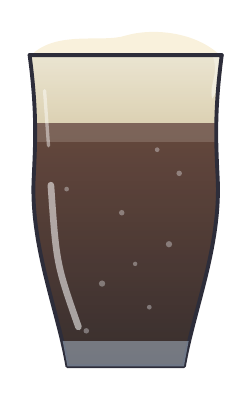
\begin{tikzpicture}[x=1cm,y=1cm, line join=round, line cap=round]
  % tulip pint: narrow foot, bulge at two thirds, flared rim
  \def\glasspath{(-0.74,0) -- (0.74,0) .. controls (0.86,0.7) and (1.2,1.5) .. (1.17,2.35)
     .. controls (1.15,2.8) and (1.12,3.2) .. (1.22,3.95) -- (-1.22,3.95)
     .. controls (-1.12,3.2) and (-1.15,2.8) .. (-1.17,2.35) .. controls (-1.2,1.5) and (-0.86,0.7) .. cycle}
  \begin{scope}
    \clip \glasspath;
    \shade[bottom color=stout, top color=stout2] (-1.4,0) rectangle (1.4,3.15);
    % the "surge" just under the head
    \fill[head, opacity=0.18] (-1.4,2.85) rectangle (1.4,3.15);
    % creamy head
    \shade[bottom color=head2, top color=head] (-1.4,3.1) rectangle (1.4,4.3);
    % rising bubbles
    \foreach \x/\y/\r in {-0.5/0.45/0.035, -0.3/1.05/0.04, 0.3/0.75/0.03, 0.55/1.55/0.04,
                          -0.05/1.95/0.035, 0.68/2.45/0.035, -0.75/2.25/0.03, 0.12/1.3/0.028, 0.4/2.75/0.03}
      \fill[white, opacity=0.35] (\x,\y) circle (\r);
  \end{scope}
  % head overflowing the rim
  \fill[head] (-1.22,3.93) .. controls (-0.9,4.28) and (-0.3,4.1) .. (0,4.2)
      .. controls (0.35,4.3) and (0.9,4.25) .. (1.22,3.93) -- cycle;
  \fill[head] (1.1,3.95) .. controls (1.2,3.7) and (1.05,3.6) .. (1.1,3.4)
      .. controls (1.18,3.5) and (1.25,3.75) .. (1.22,3.95) -- cycle;
  % glass (tinted, outlined)
  \filldraw[fill=glass, fill opacity=0.14, draw=outline, line width=1.4pt] \glasspath;
  \draw[outline, line width=1.4pt] (-1.22,3.95) -- (1.22,3.95);
  % thick base and highlights
  \fill[glass, opacity=0.45] (-0.74,0) -- (0.74,0) -- (0.8,0.32) -- (-0.8,0.32) -- cycle;
  \draw[white, line width=2.4pt, opacity=0.55] (-0.6,0.5) .. controls (-0.88,1.3) .. (-0.95,2.3);
  \draw[white, line width=1.2pt, opacity=0.45] (-0.98,2.8) -- (-1.03,3.5);
\end{tikzpicture}
\end{document}
